\setlength\parindent{0pt}

\subsection{Definitionen}

\subsubsection{Planungsproblem}
Unter einem Planungssystem für Roboter versteht man allgemein ein System, das ausgehend von einem Anfangszustand und der Beschreibung eines gewünschten Zielzustandes eine Folge von Aktionen generiert, die das betrachtete System von seinem Anfangszustand schrittweise in den gewünschten Zielzustand überführen.

\subsubsection{Aktionsplanung}
Gegeben sind Startzustand, Zielzustand und eine Menge möglicher Aktionen.
Gesucht wird eine Sequenz/eine Menge von Aktionen, die den Startzustand in den Zielzustand transformieren.

Alternativen sind das Erreichen einer Menge von Zielen, das Erreichen von Zielen mit gegebenen Einschränkungen und das Erreichen von Zielen mit gegebenen Richtlinien.

Probleme:
\begin{itemize}
	\item Teilweise unbekannte Umwelt
	\item Messunsicherheiten
	\item Effekte von Aktionen nicht immer deterministisch
	\item Externe Ereignisse können das Ergebnis beeinflussen
	\item Eigene Aktionen können das Ergebnis negativ beeinflussen
	\item Randbedingungen (Zeit, Ressourcen, etc.)
	\item Beachtung von Richtlinien
\end{itemize}

Ansatz:
\begin{itemize}
	\item Explizite Repräsentation von Zustand, Zielen, Aktionen und Plänen
	\item Flexible Planungsalgorithmen und Suchstrategien (die Ordnung des Planungsproblems ist nicht notwendigerweise die Ordnung der Planausführung)
	\item Zerlegen des Ziels (Teilziele können mehr oder weniger unabhängig erreicht werden)
\end{itemize}

Vereinfachende Annahmen:
\begin{itemize}
	\item Bekannter Ausgangszustand
	\item Deterministische Aktionen
	\item Keine externen Störungen
	\item Einfache Aktionsbeschreibung (keine bedingten, quantifizierten oder funktionale Effekte)
	\item Aktionen nur sequentiell
	\item Keine Aktionen auf Sensorik (keine Verzweigungen im Plan)
	\item Keine Zeitbeschränkung
	\item Ausreichende Ressourcen
\end{itemize}

\subsection{Suchverfahren}
Das Planen kann als Suchproblem formuliert werden, indem Anfangszustand, Zielzustände und Zieltests, Nachfolge"=Funktionen und ein optionales Gütekriterium für die Lösung definiert werden.
Lösungen des Suchproblems stellen Pfade im Zustandsraum dar.
Die verschiedenen Suchverfahren unterscheiden sich anhand ihrer Expansionsstrategien.

Bewertung:
\begin{itemize}
	\item Vollständigkeit (wenn eine Lösung existiert, wird sie auch gefunden)
	\item Optimalität (wenn eine Lösung gefunden wird, ist diese auch optimal bezüglich eines Gütekriteriums)
	\item Zeit Komplexität (wie lange dauert es eine Lösung zu finden)
	\item Raum Komplexität (wie viel Speicher wird für die Suche benötigt)
\end{itemize}

\subsubsection{Uninformierte Suche: Analytische Verfahren (Baumsuche)}
\paragraph*{Breitensuche}
\begin{enumerate}
	\item Beginn am Ausgangszustand
	\item Prüfe alle Knoten gleicher Tiefe
	\item Gehe dann eine Stufe tiefer
\end{enumerate}
Die Breitensuche ist \textbf{vollständig}.

\paragraph*{Tiefensuche}
\begin{enumerate}
	\item Beginn am Ausgangszustand
	\item Suche bis zur maximalen Tiefe
	\item Weiter im tiefsten Knoten, der noch nicht durchsuchte Kanten hat
\end{enumerate}
Die Tiefensuche ist \textbf{nicht vollständig} falls Suchraum und Suchtiefe unbeschränkt sind.

\paragraph*{Bidirektionale Suche}
\begin{enumerate}
	\item Beginne eine Breitensuche am Ausgangszustand und eine weitere am gewünschten Zielzustand
	\item Halte, wenn bei beiden Suchen ein gleicher Zustand erreicht wurde
	\item Die Lösung setzt sich aus den beiden Pfaden, mit denen dieser gleiche Zustand erreicht wurde, zusammen
\end{enumerate}
Die Bidirektionale Suche ist \textbf{vollständig}.

\paragraph*{Progression vs. Regression} \mbox{}
\vspace{1em} \\
\begin{tabular}{p{0.5\textwidth} p{0.5\textwidth}}
\textbf{Progression} (Vorwärtssuche) & \textbf{Regression} (Rückwärtssuche) \\
\begin{itemize}
	\item Wähle Aktion, deren Vorbedingungen erfüllt sind
	\item Fortfahren, bis Zielzustand erreicht ist
\end{itemize}
&
\begin{itemize}
	\item Wähle Aktion, deren Effekt ein nicht erfülltes Teilziel erfüllt
	\item Füge nicht erfüllte Vorbedingungen der Aktion zu den Teilzielen hinzu
	\item Fortfahren, bis keine unerfüllten Teilziele mehr existieren
\end{itemize}
\\
\begin{itemize}
	\item[+] Einfacher Algorithmus
	\item[-] Suche kann sehr breit werden
\end{itemize}
&
\begin{itemize}
	\item[+] Fokus auf der Erfüllung von Teilzielen
	\item[-] Regression ist unvollständig für funktionale Effekte
\end{itemize}
\end{tabular}


\subsubsection{Informierte Suche: Heuristiken}
Ist möglich, wenn zusätzliches Wissen zugänglich ist, z.B. Ignorieren irrelevanter Informationen und Ausschluss von Aktionen, die keine Annäherung zum Zielstand bringen.

\paragraph*{A*}
hat als zusätzliches Wissen die Schätzung der Distanz zwischen einem Zwischenzustand und dem gewünschten Endzustand.
A* ist eine Baumsuche mit nicht systematischer Suche entlang der Baumstruktur.
\begin{itemize}
	\item Heuristik $h(n)$: Funktion, die die Distanz (Kosten) des Zustandes $n$ zum Zielzustand schätzt
	\item Funktion $g(n)$: Ermittelt die tatsächlichen Kosten vom Ausgangszustand zum Zustand $n$
	\item Suche jeweils in dem Knoten fortsetzten, in dem $f(n) = g(n) + h(n)$ minimal ist.
\end{itemize}
A* ist \textbf{vollständig} und \textbf{optimal} falls $h(n)$ eine untere Schranke für die tatsächlichen Kosten darstellt, d.h.\ die tatsächlichen Kosten unterschätzt.

\paragraph*{Dekomposition} oder Zerlegung in unabhängige Teilprobleme.
Das zusätzliche Wissen ist die vollkommene Unabhängigkeit bestimmter Teilaufgaben.
\vspace{1em} \\
\begin{tabular}{p{0.5\textwidth} p{0.5\textwidth}}
\textbf{Linear} & \textbf{Nichtlinear} \\
\begin{itemize}
	\item Lösungen von Teilzielen werden nacheinander geplant
	\item Stack noch offener Teilziele
\end{itemize}
&
\begin{itemize}
	\item Verschachteltes Lösen der Teilziele
	\item Menge noch offener Teilziele
\end{itemize}
\\
\begin{itemize}
	\item[+] Einfache Suchverfahren
	\item[+] Effizient, wenn Teilziele unabhängig
	\item[-] Kann suboptimale Pläne erzeugen
	\item[-] \textbf{Unvollständig}
\end{itemize}
&
\begin{itemize}
	\item[+] \textbf{Vollständig}
	\item[+] Kürzere Pläne möglich
	\item[-] Größerer Suchraum
\end{itemize}
\end{tabular}

\paragraph*{Aufgabenspezifisches Wissen erforderlich}

\subsection{Lineare Planung}
\begin{itemize}
	\item Jedes Teilziel wird für sich gelöst.
	Dann Lösung des nächsten Teilziels.
	\item Teilziele auf einem Stack (feste Reihenfolge).
	\item Voraussetzung: Teilzeile sind (weitestgehend) unabhängig
	\item Lineare Planung ist effizient, wenn die Voraussetzung erfüllt ist.
\end{itemize}
Beispiel: \textbf{Blockwelt}

\subsubsection{Situationskalkül}
Das Situationskalkül benutzt ausschließlich die Prädikatenlogik 1. Ordnung zur Planung.
Sämtliche Annahmen, die von der Welt gemacht werden, müssen daher durch Axiome formuliert werden.
Das Szenenmodell ist somit eine Konjunktion von Prädikaten in Prädikatenlogik.

\begin{itemize}
	\item \textbf{Aktionen}: werden durch Funktionen dargestellt (Bsp. Blockwelt $Stack(x,y,s_t)$).
	\item Situationen: sind Zustände der Umwelt.
	Sie werden durch die Anwendung von Aktionen auf den Anfangszustand dargestellt
	\item Situationsabhängige Attribute: Die Attribute selbst werden durch Funktionen oder Variablen dargestellt.
	Ihre Auswertung wird durch das Prädikat \emph{holds(fluent,situtation)} vorgenommen.
	\item Situationsunabhängige Attribute: können einfach als Prädikate formuliert werden.
	\item \textbf{Vorbedingungen} von Aktionen: Bsp. Blockwelt $Holding(x,s_t) \wedge Clear(y,s_t)$
	\item \textbf{Nachbedingungen} von Aktionen: Bsp. Blockwelt $\neg Holding(x, s_{t+1}) \wedge Holding(nil, s_{t+1}) \wedge \neg Clear(y, s_{t+1}) \wedge On(x,y,s_{t+1} \wedge Clear(x, s_{t+1})$
	\item Ergebnisse von Aktionen: Konsequenz einer Aktion auf die folgende Situation.
\end{itemize}

\subsubsection{Blockwelt}
Operatoren
\begin{itemize}
	\item Pickup(x): Block x vom Tisch greifen
	Nach der Anwendung von $Putdown(2,s_0)$ gilt $Ontable(2,s_1)$.
	\item Putdown(x): Block x auf Tisch legen
	\item Stack(x,y): x auf y ablegen
	\item Unstack(x,y): x von y aufnehmen
\end{itemize}
Es muss nicht nur formuliert werden, was ein Operator bewirkt, sondern auch was er nicht verändert.
Die Nachbedingungen müssen also alle möglichen Nicht"=Veränderungen (Rahmenaxiome) enthalten.
Das Modellieren wird dadurch sehr lästig und das Planen darauf sehr komplex ($\rightarrow$ STRIPS).

\subsubsection{STRIPS}
= STandford Research Institute Problem Solver.
Ein linearer Planer.
Wie beim Situationskalkül haben Operatoren Vor- und Nachbedingungen.
Die Nachbedingungen bestehen jedoch aus einer \textbf{Add-} und einer \textbf{Delete"=Liste}.
Die Add"=Liste enthält diejenigen Attribute, die dem neuen Zustand durch das Ausführen der Aktion hinzugefügt werden.
Die Delete"=liste enthält diejenigen Attribute, die aus dem neuen Zustand durch das Ausführen der Aktion negiert werden.\\

Annahme: Ein Operator ändert, wenn man ihn in der Welt ausführt, genau das, was in seiner Nachbedingung angegeben ist (d.h.\ Attribute, die nicht in der Definition des Operators erwähnte werden bleiben unverändert).

\paragraph{Operator}
\begin{itemize}
	\item Operator: o
	\item Aktion: \emph{Pickup(x)}
	\item Vorbedingung: $Holding(NIL) \wedge Clear(x) \wedge Ontable(x)$
	\item Nachbedingungen:
	\begin{itemize}
		\item Add-Liste add(o): $Holding(x)$
		\item Delete-Liste del(o): $Holding(NIL), Clear(x), Ontable(x)$
	\end{itemize}
\end{itemize}

\paragraph{Planung}
\begin{itemize}
	\item Situation: Ansammlung von Fakten
	\item Planung: Suche eines Weges vom Initialzustand zum Zielzustand
	\item Ziel: Nicht ein Zielknoten, sondern eine Menge von Knoten (Ziel gibt nicht immer alles vor, bspw.\ sagt \emph{On(3,2)} nichts über Block 1 aus).
	\item [$\rightarrow$] Rückwärtssuche von der Menge der Zielknoten (\textbf{zielzentriert}) mit Mittel"=Ziel Analyse mit Zielkeller (\textbf{MZAMZK}):
	\begin{itemize}
		\item Eingabe: Menge der Ziele $Z$ und Startsituation $S$
		\item Global: Menge der Operatoren
		\item Varaible: Aktuelle Situation $St$
		\item Ausgabe: Plan $P$ (lineare Ordnung von Operatoren)
	\end{itemize}
	Wiederhole solang offene Ziele vorhanden sind:
	\begin{enumerate}
		 \item Wähle das erste Ziel $g$ aus (top of stack)
		 \item Wähle einen anwendbaren Operator $o$, dessen Add"=Liste $g$ enthält
		 \item Falls kein solcher Operator existiert dann Backtracking und weiter mit 1.
		 \item Andernfalls füge alle nicht erfüllten Vorbedingungen von $o$ zu den Zielen hinzu (push on stack)
	\end{enumerate}
	MZAMZK kann um Kritiker erweitert werden:
	\begin{itemize}
		\item Einführung eines Kritikers zum Plan"=Debugging
		\item Finden von sich aufhebenden Operationen
		\item Löschen der entsprechenden Planteile (\emph{Pickup(1)} direkt vor \emph{Putdown(1)} wird gelöscht)
	\end{itemize}
\end{itemize}

Teilzielinteraktionen:
\begin{itemize}
	\item Negative TZI: Bearbeitung eines Teilziels zerstört Teile der Bearbeitung eines anderen Ziels
	\item Positive TZI: Bearbeitung eines Teilziels erledigt Teile der Bearbeitung eines anderen Ziels mit
\end{itemize}
STRIPS berücksichtigt positive TZI, aber keine negative TZI.\\

\textbf{Sussman Anomalie} (suboptimale Pläne)
\begin{itemize}
	\item Ziel $On(1,2) \wedge On(2,3)$ (vgl. \autoref{ch06_sussman}
	\item Erzeugter Plan: \emph{Unstack(3,1)}, \emph{Putdown(3)}, \emph{Pickup(1)}, \emph{Stack(1,2)}, \emph{Unstack(1,2)}, \emph{Putdown(1)}, \emph{Pickup(2)}, \emph{Stack(2,3)}, \emph{Pickup(1)}, \emph{Stack(1,2)}
	\item Die Sussman Anomalie kann mit POP (\autoref{ch06_nichtlinearePlanung}) oder Einführung eines Kritikers gelöst werden.
\end{itemize}

\begin{figure}[ht]\centering 
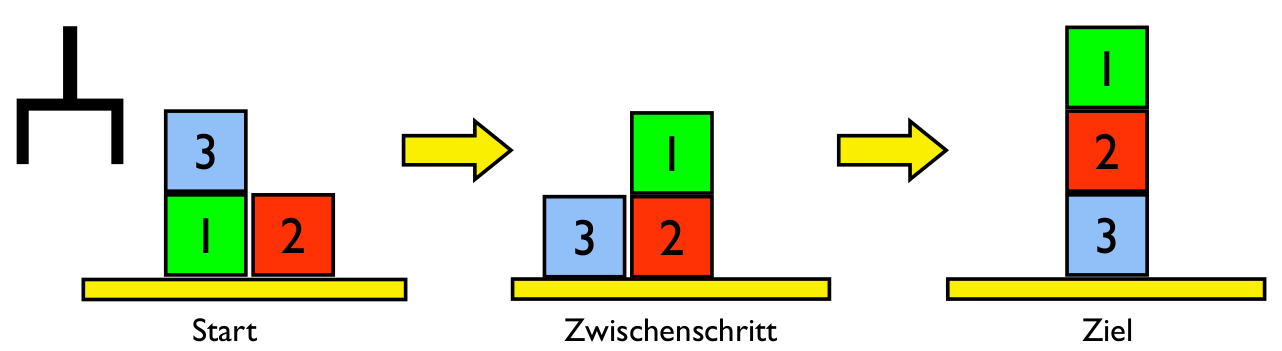
\includegraphics[width=\textwidth]{figures/ch06_sussman.png}
\caption{Sussman Anomalie}
\label{ch06_sussman}
\end{figure}

\textbf{One way Rocket-} und Zuweisungs"=Problem (unlösbare Probleme):
\begin{itemize}
	\item Geg.: zwei Objekte $o_1$ und $o_2$, Flugzeug $p$ und Flughafen $a_1$
	\item Aktionen: $load(a,o,p)$ und $unload(a,o,p)$
	\item Ziel: $at(a_2, o_1$, $at(a_2, o_2)$
	\item definiere: $fly(p,a_1,a_2)$ mit
	\begin{itemize}
		\item Precond: $plane(p) \wedge at(p,a_1) \wedge haveFuel(p)$
		\item Add: $at(p,a_2)$
		\item delete: $at(p,a_1), haveFuel(p)$
	\end{itemize}
	\item[$\rightarrow$] kann mit linearer Planung nicht gelöst werden, da immer ein Teilziel vollständig erfüllt wird und damit die Vorbedingung für das zweite Ziel nicht mehr gegeben ist
\end{itemize}

\subsubsection{Diskussion}
Vorteile:
\begin{itemize}
	\item Reduzierter Suchraum, weil Teilziele nacheinander gelöst werden
	\item Vorteile, wenn Teilziele unabhängig
	\item Produziert nur gültige Pläne
\end{itemize}
Nachteile:
\begin{itemize}
	\item Kann suboptimale Pläne erzeugen
	\item ist unvollständig
\end{itemize}

\subsection{Nichtlineare Planung}
\label{ch06_nichtlinearePlanung}
Planung als Suche mit einer (Teil-)Ziel"=Menge (statt Stack). Arbeite mit einer Menge von Zielen.
Im Suchraum werden alle möglichen Teilziel"=Anordnungen dargestellt: Teilzielinteraktionen durch Ziel"=Verzahnung bei der Planung betrachtet.
Abhängigkeiten der einzelnen Operatoren können geplant werden.
Plan kann z.B.\ in Form eines Vorranggraphen gespeichert werden.
NLP folgt \textbf{Least Commitment Strategie} (Prinzip der geringsten Festlegung):
\begin{itemize}
	\item Es gibt keine a priori Festlegung der Reihenfolge, in der die Ziele erreicht werden sollen
	\item Die Reihenfolge, in der Aktionen ausgeführt werden, wird nur soweit nötig festgelegt
	\item Variablen werden nur falls notwendig instanziiert
\end{itemize}

Vorteile:
\begin{itemize}
	\item Erzeugt nur gültige Pläne
	\item vollständig
	\item Optimalität bzg.\ irgendeines Kriteriums kann erreicht werden
\end{itemize}
Nachteile:
\begin{itemize}
	\item Größerer Suchraum, alle Teilzielreihenfolgen müssen beachtet werden
	\item Komplexere Algorithmen
\end{itemize}

Ein nicht"=linearer Plang $P$ ist eine Datenstruktur mit folgenden Komponenten:
\begin{itemize}
	\item eine Menge von Planschritten $S$ mit Operation $o$ ($S:o$)
	\item eine Menge von Ordnungsbedingungen, die die Reihenfolge von Planschritten angeben ($S_i < S_j$), d.h.\ \glqq $S_i$ vor $S_j$ \grqq
	\item eine Menge von Variablenbedingungen ($x=t$), wobei $x$ eine Variable und $t$ ein Term ist, und Ungleichungsbeschränkungen
	\item eine Menge von kausalen Beziehungen (causal links), die Zusammenhänge zwischen Planschritten beschreiben, d.h.\ $S_i$ erzeugt die Vorbedingung $c$ für $S_j$
	\item Menge der offenen Vorbedingungen
\end{itemize}

\subsubsection{Einfacher Algorithmus}
Wiederhole solange Zielmenge $G$ nicht leer ist
\begin{itemize}
	\item Wähle $g$ aus $G$
	\item Wenn $g$ nicht im Zustand enthalten ist
	\begin{itemize}
		\item Wähle Operator $o$, dessen Add-Liste $g$ enthält
		\item Füge $o$ zu den auszuführenden Operationen hinzu
		\item Füge Vorbedingungen von $o$ zu $G$ hinzu
	\end{itemize}
\end{itemize}

\subsubsection{Partial Order Planning (POP)}
POP basiert auf einer Suche im Raum der mögliche Pläne, nicht auf einer direkten Suche im Zustandsraum.
\begin{figure}[ht]\centering 
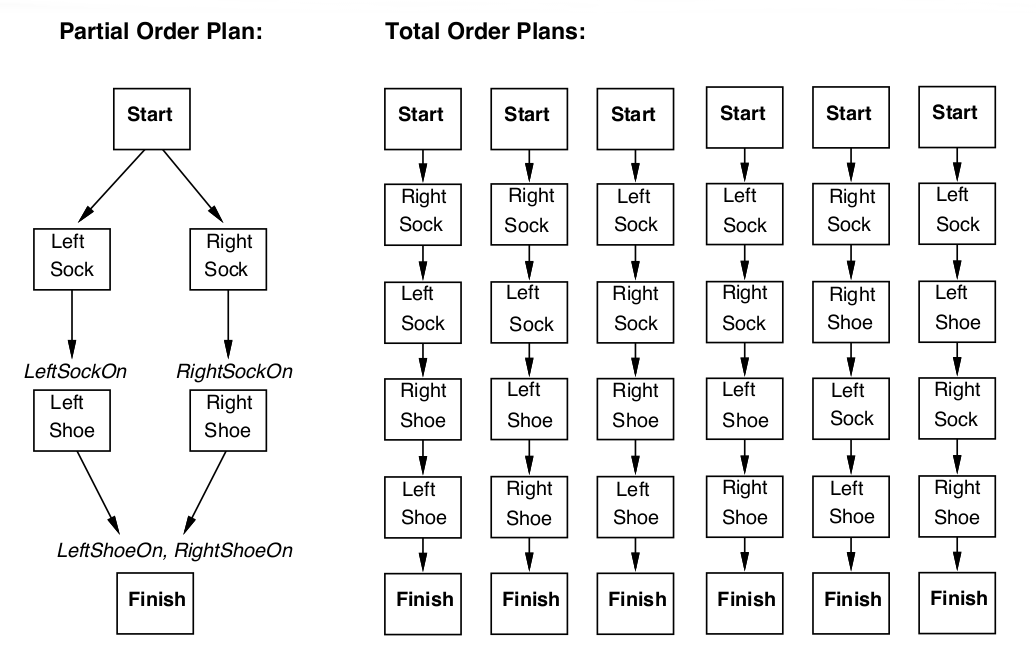
\includegraphics[width=\textwidth]{figures/ch06_partialOrder.png}
\caption{Partial vs.\ Total Order Planning (bei linearer Planung)}
\label{ch06_orderPlanning}
\end{figure}
\begin{itemize}
	\item Knoten: (unvollständige) Pläne
	\item Kanten: Planmodifikationsschritte
	\begin{itemize}
		\item Einfügen von Planschritten
		\item Anordnen von Planschritten
		\item Instanziieren von Variablen
	\end{itemize}
\end{itemize}
POP ist \textbf{vollständig} und erzeugt konsistente nicht"=lineare Pläne. 
Jede Linearisierung eines solchen Plans ist eine Lösung des Planungsproblems.

\begin{figure}[ht]\centering 
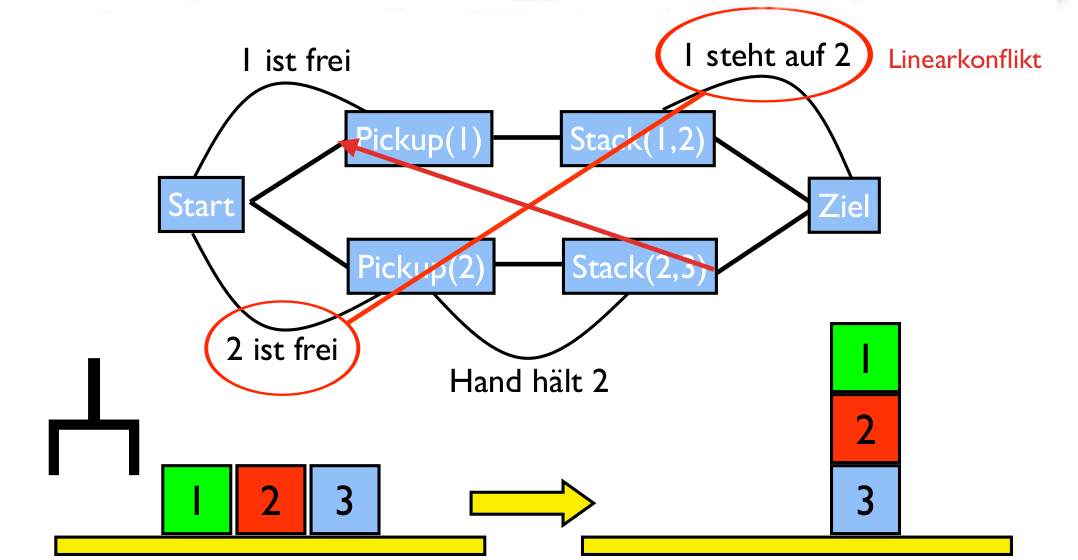
\includegraphics[width=0.7\textwidth]{figures/ch06_popKonflikte.png}
\caption{POP Konflikte}
\label{ch06_popKonflikte}
\end{figure}

Kritiker: nach der Konfliktauflösung (\autoref{ch06_popKonflikte}) den Plan weiter optimieren, bspw.\
\begin{itemize}
	\item Redundante Kanten entfernen
	\item Operatoren löschen, von denen keine Abhängigkeiten ausgehen
	\item Hilfreiche Interaktionen entdecken
	\item Umwege entfernen (siehe Sussman"=Anomalie)
\end{itemize}

\subsubsection{Total vs.\ Partial Order Planning}
\begin{tabular}{p{0.5\textwidth} p{0.5\textwidth}}
\textbf{Total Order} & \textbf{Partial Order}\\
\begin{itemize}
	\item Plan entspricht immer einer strikten Sequenz von Aktionen
\end{itemize}
&
\begin{itemize}
	\item Aktionen können ungeordnet sein
	\item Nur notwendige Abhängigkeiten werden geplant
	\item Plan muss evtl.\ vor der Ausführung linearisiert werden
\end{itemize}
\\
\begin{itemize}
	\item[+] Einfachere Algorithmen
	\item[-] Keine nebenläufigen Pläne
	\item[-] Enthält evtl.\ unnötige Abhängigkeiten
\end{itemize}
&
\begin{itemize}
	\item[+] Enthält nur notwendige Abhängigkeiten
	\item[+] Nebenläufige Pläne darstellbar
	\item[-] Feststellung der erfüllten Teilziele zu einem Zeitpunkt schwierig
	\item[-] Komplexere Darstellung
\end{itemize}
\end{tabular}


\subsection{Hierarchische Planung}
Hierarchische Aufgabennetzwerke (Hierarchical Task Networks, HTN), Planung in Dimension der Abstraktion.
\begin{itemize}
	\item Komplexe Pläne haben meistens erkennbare Strukturen
	\item Diese Struktur kann oft in Form von Hierarchien ausgedrückt werden
	\item Teilpläne sind oft voneinander unabhängig
	\item Hierarchische Planung versucht die Dimensionalität des Problems zu reduzieren, im Gegensatz zur vollständigen Suche im Plan- oder Zustandsraum
\end{itemize}

Klassische Planung kombiniert elementare Operationen, hierarchische Planung entfaltet abstrakte Operationen (vgl.\ \autoref{ch06_hierarchischePlanung}).

\begin{figure}[ht]\centering 
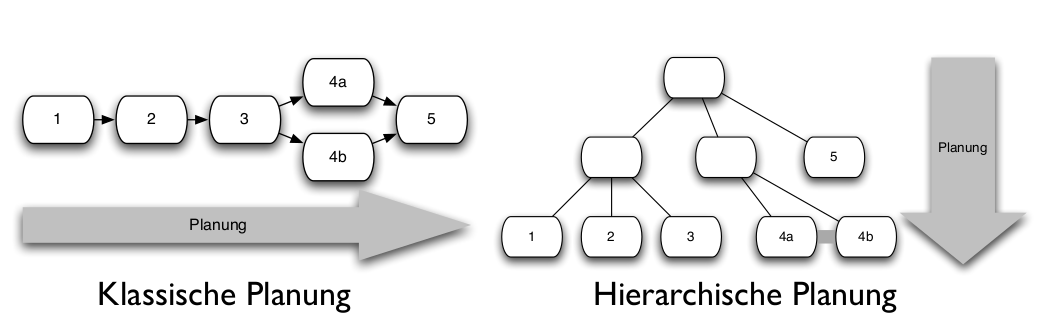
\includegraphics[width=0.8\textwidth]{figures/ch06_hierarchischePlanung.png}
\caption{Unterschiedliche Planungsrichtungen für klassische Planung und hierarchische Planung}
\label{ch06_hierarchischePlanung}
\end{figure}

Ein abstrakter Plan enthält \underline{zusammengesetzte Operatoren}:
\begin{itemize}
	\item Vorbedingungen, Effekte
	\item Methoden zur Zerlegung in Teilpläne
	\begin{itemize}
		\item Aufbau der Teilplanstruktur
		\item Parameter
		\item Ähnliche Funktionsaufrufe
	\end{itemize}
\end{itemize}
Ein voll instantiierter Plan besteht nur aus \underline{Primitiven Operatoren}:
\begin{itemize}
	\item STRIPS"=ähnliche Beschreibung
	\item keine Vorbedingungen
\end{itemize}

\subsubsection{Suchraum}
\begin{itemize}
	\item Ziel ist eine abstrakte Aufgabe (Task), nicht ein Weltzustand (State)
	\item Operatoren im Suchraum
	\begin{itemize}
		\item Zerlegung in Teilpläne
		\item Parametrisierung
		\item Konfliktlösung
	\end{itemize}
	\item Algorithmus HTN"=Planung:
	\begin{itemize}
		\item Starte mit initialer abstrakter Aufgabe (nicht Weltzustand/Zielliste!!)
		\item Baue das Aufgabennetzwerk durch wiederholtes Expandieren in Teilpläne auf, bis der Plan voll instantiiert ist
		\item Expandieren durch Verwendung von Methoden, deren Anwendbarkeit gegeben ist
	\end{itemize}
\end{itemize}

\subsubsection{Simple Hierarchical Order Planner (SHOP)}
\paragraph{SHOP Algorithmus}
\begin{itemize}
	\item Vorwärtssuche, lineare Planungsverfahren
	\begin{itemize}
		\item Planung in Ausführungsreihenfolge
		\item Tiefensuche
	\end{itemize}
	\item Elementaroperatoren haben keine Vorbedingungen
	\item Keine parallelen Aktionen
	\item Sehr mächtige Operatorrepräsentation
	\item Effizienter Planungsalgorithmus
	\item Korrekt und vollständig
\end{itemize}
\paragraph{Stärken des Algorithmus}
\begin{itemize}
	\item Methoden codieren Domänenwissen
	\item Methoden beinhalten Problemlösungswissen
	\item Abstraktion kapselt Operatorinteraktionen
\end{itemize}
\paragraph{Nachteile}
\begin{itemize}
	\item Immer noch NP-vollständig
	\item Terminiert nicht zwangsläufig (rekursives Anwenden von Methoden, Endlosschleifen sind evtl.\ schwer zu detektieren!)
	\item Plan kann erst im voll expandierten Zustand bewertet werden $\rightarrow$ Konflikte können evtl.\ erst dann entdeckt werden
\end{itemize}
\paragraph{Mögliche Erweiterungen}
\begin{itemize}
	\item Erkennung/Lösung von Konflikten
	\begin{itemize}
		\item Teilzielinteraktion
		\item Mehrfachverwendung/Wiederverwendung von Operatoren
	\end{itemize}
	\item Methoden beinhalten Vorbedingungen und Effekte
	\begin{itemize}
		\item Konflikte in der Planungsphase erkennen
	\end{itemize}
	\item Methoden beinhalten Ressourcenangaben
	\begin{itemize}
		\item Scheduling
	\end{itemize}
\end{itemize}